\documentclass[12pt,titlepage,twoside]{report}
% font
\usepackage{dejavu}
\usepackage{sectsty}
\allsectionsfont{\sffamily}
% language stuff
\usepackage{german, ngerman}           % deutsche Überschriften etc.
\usepackage[utf8]{inputenc} % direkte Einbgabe von Umlauten
% miscellaneous
\usepackage{graphicx}         % graphics
\graphicspath{{grafiken/}}
\usepackage[german]{fancyref}
\usepackage{hhline}           % double lines in tables
\usepackage{amsfonts}         % real numbers etc.
\usepackage[rightcaption]{sidecap} % figure captions on the right (optional)
\usepackage{hyperref}         % for URLs
\usepackage{listings}         % for code samples
\usepackage{fancyhdr}         % for header line
\usepackage[backend=biber, style=authoryear-icomp]{biblatex}
\addbibresource{literatur.bib}
% \usepackage{natbib}
% Hier bei Bedarf die Seitenränder einstellen

\usepackage[printonlyused]{acronym}

\usepackage{algorithm}

% Kopf- und Fußzeile
\fancyhead{} % clear all header fields
\fancyhead[RO,LE]{\leftmark}

\title{Arbeit}
\author{Alexander Martin}
\date{August 2021}

\begin{document}

\begin{titlepage}
  \begin{center}
    {\Large\bf Entwurf und Implementierung einer generischen Ingestion-Schnittstelle mit Versionierung für Data-Lake-Systeme}\\[2cm]

    {\bf Masterarbeit}\\
    zur Erlangung des Grades {\em Master of Science}\\[1cm]

    an der\\
    Hochschule Niederrhein\\
    Fachbereich Elektrotechnik und Informatik\\
    Studiengang {\em Informatik}\\[2cm]

    vorgelegt von\\
    Alexander Martin\\
    1018332\\[3cm]
    Datum: \today\\[2cm]

    Prüfer: Prof.~Dr.~rer.~nat.~Christoph Quix\\
    Zweitprüfer: Sayed Hoseini,~M.Sc.

  \end{center}
\end{titlepage}
\newpage
\include{unabhänhigkeit}
\newpage
\section*{Zusammenfassung}

Heutzutage spielen Daten eine immer wichtiger Rolle.
Durch den vermehrten Einsatz von IoT-Geräten und moderne Cloud-Speicher-Lösungen, wächst die Zahl an anfallenden Daten vielen Firmen und Forschungseinrichtungen stetig.
Mit steigenden Datenmengen und der diversen Strukturen der Daten ist deren Verwaltung ein komplexes Thema geworden.
Diese Arbeit befasst sich mit der technischen Herausforderung Daten aus verschiedensten Quellen zu Verwalten.
Als Lösung hierfür wurden Data-Lake-Systeme vorgeschlagen.
Im Kontext des HIT-Institut der Hochschule Niederrhein, wurde ein Prototyp für einen Data-Lake entwickelt.
In dieser Arbeit wird eine Schnittstelle entwickelt, über die Benutzer Daten aus unterschiedlichen Quellen in dieses System laden können.
Dabei werden Metadaten über die Datenquellen gesammelt.
Mit der Schnittstelle ist es auch möglich, die geladenen Daten zu versionieren, um weiter Verarbeitungen effizienter zu machen.

\section*{Abstract}

In todays world data play an important role.
The amount of data in comapnies and research facilities is growing due to the increasing use of IoT-devices and modern Cloud-Storage-Solutions.
With the bigger amount of data and their varying structures the data management got more complex.
This thesis takes on the technical challenge of managing data from different sources.
Data lakes are a proposed solution for this problem.
A prototype for a data lake was developed at the HIT-institute at the Hochschule Niederrhein.
This thesis devolopes an interface for users to ingest data from diffenrent sources to the system.
The interface collects metadata about the data sources.
It is also capable of saving data with versioning to make further processing more efficient.
\newpage

\pagestyle{fancy}
\tableofcontents
\newpage

\chapter{Einleitung}

\section{Die Motivation}
In der heutigen Zeit spielen Daten in der Welt eine immer größere Rolle.
In \textit{Rethink Data Report 2020} \textcite{rethink_data_2020} wurde eine Studie durchgeführt, die eine Steigerung von 42\% der Menge an anfallenden Daten pro Jahr prognostiziert.
Dies wird unter anderem auf den vermehrten Einsatz von IoT-Geräten, immer ausführlicheres Analysieren von Daten und die einfacher werdende Anwendung von Cloud-Speichern zurückgeführt.
Dabei besteht die Herausforderung, Daten in verschiedensten Formaten in großen Mengen zu verwalten und zu verwenden.

Ein Lösungansatz für dieses Problem sind Data-Lake-Systeme.
Data-Lake-Systeme sind zentrale Datenspeicher, die strukturierte, semi- und unstrukturierte Daten in ihrem Rohformat speichern.
Mit Hilfe von Metadaten bietet ein Datalake Schnittstellen zur Datenanalyse und -abfrage.
Dabei funktioniert das System nach dem Schema-On-Read oder auch ELT (Extrahieren Laden Transformieren) Prinzip.
Das bedeutet, dass die Daten wie bereits erwähnt im Rohformat im Data Lake gespeichert werden und erst nach dem Laden ein entsprechendes Schema angewendet wird.

Es gibt bereits viele Anbieter, die fertige Data-Lake-Systeme anbieten.
Dabei ist jedoch ein Nachteil, dass sie häufig nur in der (Cloud-)Infrastruktur des Anbieters (z.B. Microsoft Azure\footnote{https://azure.microsoft.com/}, Amazon Web Services\footnote{https://aws.amazon.com/}) verfügbar sind und sich ihrere Architektur nach diesen Diensten richtet.
Daher wird in dieser Arbeit eine Schnittstelle für die Ingestion, also das Laden der Daten in das Data-Lake-System, entwickelt, die in einem platform unabhängigen Data-Lake-System Anwendung finden soll.

\section{Der Aufbau}
Am Anfang wird auf die Ziele eigengangen, die Schnittstelle erreichen soll.
Aus diesen Zielen werden dann konkrete Anforderungen an die Entwicklung abgeleitet.
Im zweiten Kapitel wird das System der Schnittstelle entwickelt, ohne dabei auf konkrete Details, wie zum Beispiel Programmiersprachen, einzugehen.
Hier geht es mehr um die Architektur und das Design, das benötigt wird um alle Anforderunegn abzudecken.
Danach wird die Umsetzung beschrieben.
Hierbei spielt vorallem das bereits exisitierende Data-Lake-System, in dem die Ingestion-Schnittstelle integriert werden soll, eine große Rolle.
Zum Schluss wird die Ingestion-Schnittstelle evaluiert und ein Ausblick auf mögliche weitere Arbeiten gegeben.

\section{Das Existierende System}
In dem Masterprojekt \textit{Development of a Data Lake System} \parencite{datalake_proj} an der Hochschule Niederrhein wurde bereits eine Data-Lake-System-Prototyp entwickelt.
Das System ist eine monolithische Client-Server-Anwendung.
Es besteht aus einer REST-API, die zur Interaktion mit dem Data-Lake-System verwendet wird und einem Web-Frontend.
Außerdem können durch einfach Anpassungen der Server-Anwendung beliebige Datenspeicher in das Data-Lake-System integriert werden.

Als Basis wird \textit{Apache Spark}\footnote{https://spark.apache.org/} verwendet.
\textit{Apache Spark} ist eine Plattform, um Analyse auf großen Datenmengen aus zu führen.
Außerdem gibt es Schnittstellen für \textit{Scala, Java und Python} und es wird auch die Verarbeitung von Datenströmen und maschinelles Lernen unterstützt \parencite{spark}.

Der Server ist in \textit{Python} geschrieben und verwendet das Framework \textit{Flask}\footnote{https://palletsprojects.com/p/flask/} um eine REST-API bereitzustellen, über die mit dem Data Lake interagiert werden kann.
Dabei werden über die API \textit{JSON}-Objekte ausgetauscht, so dass die API client-unabhängig verwendet werden kann.
Der Client des Projekts ist eine Webanwendung, die mit \textit{Angular}\footnote{https://angular.io/} umgesetzt wurde.

\section{Verwandte Arbeiten}

\chapter{Entwicklung}
In diesem Kapitel werden die einzelnen Komponenten, die für eine komplette Ingestion notwendig sind entwickelt.
Nach \citeauthor{DL-Ing-Mgmt} ist der Ingestion-Prozess eines Data-Lake-Systems, als erster Schritt im Lebenszyklus der Daten, maßgebend dafür, wie gut die Daten später verwendet und verarbeitet werden können.
Dafür sollte das System einige Herausforderungen erfüllen.
Diese sind die Unterstützung für strukturiert, teil-strukturiert und unstrukturierte Datenquellen und die Möglichkeit für einmalige oder kontinuierliche Ingestion.
Zu dem zweiten Punkt gehört außerdem, dass geänderte Daten mit einer Datenversionierung im Data Lake gespeichert werden können.
Zur Erfüllung dieser Herausforderungen und um allgemein gut mit den Daten interagieren zu können, sollte sich die Ingestion zusätzlich um die Erstellung von Metadaten kümmern.

Das zu entwickelnde System lässt sich in die drei Teile Ingestion, Delta-Erkennung und Datenversionierung unterteilen.
Bei der Ingestion soll der Teil entwickelt werden, der dafür verantwortlich ist, Daten aus verschiedensten Quellen in das Data-Lake-System zu laden und zu speichern.
Die Delta-Erkennung ist ein Mechanismus, der dafür sorgen soll, dass bei einer kontinuierlichen Ingestion nur geänderte Daten neu in das System integriert werden.
Zum Schluss hat die Datenversionierung das Ziel, geänderte Daten im Data Lake so zu verwalten, dass Analysen über den Verlauf der Daten und Abfragen älterer Version möglich werden.

\section{Vorüberlegungen}

\subsection{Datenquellen}
Ein Kernpunkt für die Entwicklung der Ingestion-Schnittstelle ist die Analyse der möglichen Datenquellen.
Da das System alle möglichen Datenquellen unterstützen soll, werden hier mögliche Typen dargestellt, mit denen sich alle Datenquellen abdecken lassen.
Dazu werden Merkmale betrachtet die Art und der Typ Ingestion bestimmen.
Mit der Art wird hier bezeichnet, ob die verwendeten Daten strukturiert, semi- oder unstrukturiert sind.
Da in der Vorarbeit, dem Masterprojekt, \textit{Apache Spark} verwendet wurde, ist dieser Punkt bereits abgedeckt und fällt bei der Entwicklung nicht weiter ins Gewicht.

Als zweites gibt es die Typen, die hier beschreiben, wie Daten in das System gelangen.
Dazu gibt es zwei Merkmale, in denen sich die Ingestions unterscheiden können.
Das erste ist, ob die Unterscheidung zwischen Push- und Pull-Prinzip.
Bei dem Push-Prinzip werden die zu speichernden Daten mit der Anfrage an das System gesendet und bei dem Pull-Prinzip muss dass System die Daten aus einer Quelle laden.
Die zweite Unterscheidung findet statt in einmalige in kontinuierliche Ingestion.
Diese Unterscheidungen können, müssen aber nicht, von der Datenquelle abhängig sein.
Als Beispiel gibt es Datenströme, die laufend Daten senden und somit eine Ingestion benötigen, die auch laufend Daten annimmt.
Im Gegensatz dazu gibt es Datenbanken, bei denen das System die Daten aus der Quelle laden muss und somit die Ingestion sowohl einmalig als auch kontinuierlich sein kann.

Aus diesen Unterscheidungen ergeben sich die vier mögliche Verarbeitungswege, die in \ref{fig:ingestion_types} zu sehen sind.
Sowohl für Push- und Pull-Prinzip kann eine einfache Ingestion ausgeführt werden, die sich für kontinuierliche Pull-Ingestions wiederholt.
Bei einer kontinuierlichen Ingestion, bei der Daten an das System gesendet werden, handelt es sich um Datenströme, die eine extra Verarbeitung erfordern.

\begin{figure}
    \centering
    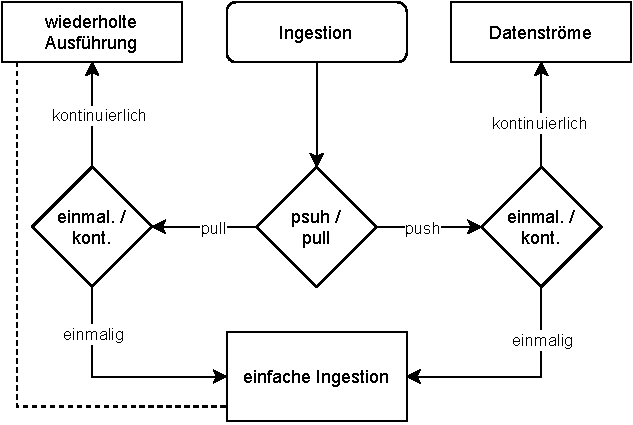
\includegraphics{Grafiken/ingestion-types.pdf}
    \caption{Ingestion-Typen}
    \label{fig:ingestion_types}
\end{figure}

\subsection{Architektur Ansatz}
Die Anwendung, die im Masterprojekt entwickelt wurde ist eine monolithische Anwendung.
Das bedeutet, dass die gesamte Software als ein großes Programm entwickelt und bereitgestellt wird.
Solche Anwendungen sind zwar in der Entwicklung und Bereitstellung leicht umzusetzen, haben aber größere Nachteile in Bereichen wie Fehlertoleranz und Wartung.
Im Vergleich dazu gibt es die Microservice-Architektur, bei der mehrere kleine Anwendungen entwickelt werden, die bestimmte aufgaben übernehmen und am gesamt Problem gemeinsam beteiligt sind.
Diese haben im, wie von \textcite{microservices} dargestellt, mehrere Vorteile gegenüber monolithischen Anwendungen.
Die Wartung fällt bei vielen kleinen Programmen leichter, da sie übersichtlicher und verständlicher sind als ein großes und Fehler betreffen jeweils nur den Microservice selbst.
Außerdem ist es einfacher bestimmte Aspekte der Software zu skalieren und bei Updates bleibt eine höhere Verfügbarkeit, da nur ein kleiner Teil des Systems neu gestartet werden muss.

Als Nachteil wird aber auch erwähnt, dass die Bereitstellung einer Mircoservice-Architektur komplexer ist als die einer monolithischen.
Diese Problem kann aber mit Container-Lösung wie \textit{Docker}\footnote{https://www.docker.com/} vereinfacht werden.
Dabei werden sogenannte Contianer aus den Mircoservices gebaut, die ähnlich zu einer virtuellen Maschine sind und einen bestimmten Zustand speichern.
Beim Starten eines Containers wird genau in diesem Zustand eingestiegen, so dass man ohne großen Aufwand zum Beispiel einen Webserver mit einer bestimmt Anwendung auf verschiedenen System starten kann, ohne sich um deren Installationen kümmern zu müssen.

Auf Grund der genannten Vorteile soll das Data Lake System und damit die Ingestion als Microservice-Architektur entwickelt werden.
Das bedeutet, dass Punkte gefunden werden müssen, an denen sich das System gut in einzelene Anwendungen trennen lässt.

\section{Ingestion}
Bei der Entwicklung der Ingestion wird das Laden der Daten und die Architektur der Anwendung betrachtet.
Es wird eine Datenmodell, in dem die Informationen zu den Datenquellen gespeichert werden, der Ablauf der verschiedenen Ingestion-Prozesse und die Kommunikation zwischen den einzelnen Mircoservices entwickelt.

\subsection{Server Architektur}
\label{sec:arch}

\begin{figure}
    \centering
    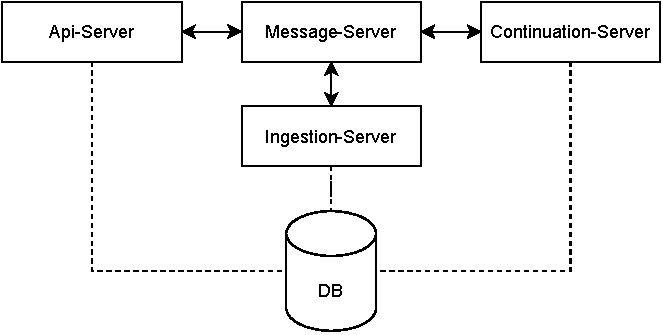
\includegraphics{Grafiken/ingestion-arch.pdf}
    \caption{Architektur der Ingestion Komponenten}
    \label{fig:ingestion_arch}
\end{figure}

Für die Umsetzung der Mircoservice-Architektur wird die Ingestion in Komponenten aufgeteilt, die \fref{fig:ingestion_arch} zu sehen sind.
Es gibt drei Services, die für die Ingestion spezifischen Aufgaben zuständig sind, eine Datenbank, in der die Informationen über Datenquellen gespeichert werden und einen Service, der für die Kommunikation verantwortlich ist.
Der \textbf{Api-Server} bietet einen REST-Schnittstelle, über die man mit der Ingestion interagieren kann.
Hier werden die Endpunkte aus \fref{tab:enpoints} benötigt, die die Schnittstellen zur Verwaltung von Datenquellen und das Ausführen von Ingestions bereitstellen.
Außerdem ist er dafür zuständig, die empfangenen Informationen über Datenquellen in der Datenbank zu verwalten.
der \textbf{Continuation-Server} überprüft regelmäßig alle kontinuierlichen Datenquellen, ob diese eine Zeitsteuerung haben und aktuell ausgeführt werden sollten.
Der \textbf{Ingestion-Server} ist die Anwendung, die die eigentliche Ingestion ausführt.
Dafür wartet dieser auf eine Aufforderung durch entweder den Api- oder den Continuation-Server.

\begin{table}[!ht]
    \centering
    \begin{tabular}{| l | l | p{3in} |}
        \hline
        Pfad                                        & HTTP-Methode  & Beschreibung \\
        \hline \hline
        /datasources                                & GET           & Liefert alle im System gespeicherten Datenquellen \\
        \hline
        /datasources/\textless id\textgreater       & GET           & Liefert die Datenquelle mit der im Pfad übergebenen Id \\
        \hline
        /datasources                                & POST          & Erstellt eine neue Datenquelle \\
        \hline
        /datasources/\textless id\textgreater       & PUT           & Bearbeitet die Daten Datenquelle mit der im Pfad übergebenen Id \\
        \hline
        /datasources/\textless id\textgreater/run   & GET           & Startet eine Ingestion der Datenquelle mit der im Pfad übergebenen Id \\
        \hline
    \end{tabular}
    \caption{Endpunkte des Api-Servers}
    \label{tab:enpoints}
\end{table}

\subsection{Plugins}
Da bei manchen Ingestions nicht immer ein festgelegtes Vorgehen ausreicht, um die Daten aus bestimmten Datenqellen zu laden, muss ein System entwickelt werden, wie möglichst ohne großen Aufwand die Inegstion erweitert werden kann.
Beispiele für solche Fälle sind die Verarbeitung von Datenströmen oder die Ingestion von Daten aus APIs, die nicht generallisiert werden können.
Als Lösung für das Problem, können Plugins der Datenquelle hinzugefügt werden. 
Diese Plugins sollen Logik enthalten, die an verschiedenen Stellen der Ingestion ausgeführt werden sollen.
Aktuell sind diese Stellen das Laden der Daten, nach dem Laden der Daten und die Stream-Verarbeitung.
Dabei ist zu beachten, dass Plugins, die das Laden der Daten abhandeln, das Standardverhalten des Ingestion-Servers überschreiben und das Stream-Verarbeitung nur mit Plugins möglich ist.
Damit es nicht zu Konflikten bei Abhängigkeiten der Plugins gibt, muss der Ingestion-Server eine Mechanik implementieren, bei der die Abhängigkeiten der Plugins für jede Datenquelle dynamisch gealden werden.

\subsection{Datenquellen}
Eine letzte Vorüberlegung für die Ingestion ist, welche Informationen erfasst werden müssen, um eine generische Ingestion zu ermöglichen.
Da es keine klaren Parameter wie zum Beispiel Datenbanknamen oder IP-Adressen gibt, die bei allen Quellen gleich sind, orientiert sich die Eingabe an der Funktionsweise von \textit{Pyspark / Apache Spark}.
Um festzulegen, woher Daten gelesen werden sollen, kann man beim erstellen einer \verb|SparkSession| einmal das Format der zu lesenden Daten angeben.
Außerdem bietet die \verb|SparkSession| die Funktion Maven-Abhängigkeiten hinzuzufügen, die Unterstützung für verschiedene Formate bringen.
Bei den meisten Formaten müssen zusätzlich noch Optionen gesetzt werden, die zum Beispiel Verbindungsparameter oder Lesemodus enthalten.
Diese Optionen sind eine Sammlung von Schlüssel-Wert-Paaren.
Eine Ausnahme besteht hierbei bei der Optionen, für die Quelledateien bei Datei-Ingestions, da diese automatisch durch die Anwendung gesetzt wird.
Daraus lassen sich bereits drei Felder ableiten, die in einem Datenmodell für die Datenquellen enthalten sein müssen: Format, Pakete und Optionen.

Neben den \textit{Spark}-spezifischen Feldern soll die Datenquelle auch die anwendungsspezifischen Informationen enhalten.
Dazu gehören Informationen über den Typ der Ingestion (siehe \ref{fig:ingestion_types}), Zeitpunkt der Erstellung und Aktualisierung, Plugins und Quelldateien und die mögliche Zeitsteuerung der Inegstions.


\section{Deltaerkennung}

\chapter{Umsetzung}

Bei der Umsetzung ist die erste Frage, die zu klären ist, mit welcher Programmiersprache gearbeitet werden soll.
In diesem habe ich mich aus verschiedenen Gründen für \textit{Python} entschieden.
Der erste ist, dass \textit{Python} bereits im Masterprojekt verwendet wurde und so die Integration leichter fällt.
Als zweites geht es speziell um die Bibliothek \textit{PySpark}.
\textit{PySpark} ist die Bibliothek, mit deren Hilfe \textit{Apache Spark} in \textit{Python} verwendet werden kann.
Neben \textit{PySpark} gibt es auch Bibliotheken für die Sprachen \textit{Java} und \textit{Scala}.
Der entscheidende Unterschied hierbei ist aber, dass \textit{Python} eine interpretierte Sprache ist.
Das bedeutet, dass der geschrieben Programmcode nicht in Maschinensprache übersetzt wird, sondern durch einen sogenannten Interpreter ausgeführt.
In diesem Anwendungsfall hat das den Vorteil, dass die Spark-Jobs nicht als kompilierte jar-Datei explizit ausgeführt werden müssen, sondern der Interpreter sich an den entsprechenden Zeitpunkten um die Ausführung kümmert.
Das bedeutet, dass die Konfiguration eines Spark-Jobs dynamisch während der Ausführung des Programms gemacht werden kann und man so mehr Freiheit für die Entwicklung bekommt.
Der letzte Vorteil ist, dass Programmcode dynamisch aus Dateien nachgeladen werden kann, was für die Umsetzung der Plugins wichtig ist.

\section{Voraussetzungen}
Um das Datalake System umsetzen zu können müssen einige Voraussetzungen erfüllt sein.
Die erste ist, wie in \ref{fig:ingestion_arch} bereits beschrieben, dass ein Server benötigt wird, der sich um die Verteilung von Nachrichten kümmert.
Als zweites muss außerdem ein zentraler Speicher für Dateien bereit stehen, indem sowohl Datenquelldateien als auch Plugindateien abgelet und von jedem Server abgerufen werden können.

\subsection{Apache Kafka}

\textit{Apache Kafka} ist ein verteiltes Event-Streaming-System, dass nach dem Publish-Subscribe-Muster funktioniert.
Events können von Produzenten in das System veröffentlicht werden und Konsumenten können diese Events abonnieren.
Das ganze läuft dabei in Echtzeit ab.
Durch seine Verteilung kann \textit{Kafka} den Ausfall einzelner Server ausgleichen.
Außerdem können Ströme von Events für einen beliebigen Zeitraum abgespeichert werden.

\textit{Kafka} besteht aus einem Cluster von Servern und verschiedenen Clients.
Es gibt zwei Arten von Servern.
Einige bilde die Speicherebene von \textit{Kafka} und werden Broaker genannt.
Die anderen verwenden \textbf{Kafka Connect}\footnote{https://kafka.apache.org/documentation/\#connect} um extierende Systeme, zum Beipsiel eine Datenbank, in das Kafka Cluster zu integrieren.
Anwendungen, die entweder Events produzieren oder konsumieren sind die Clients.

In diesem System repräsentiert ein Event den Fakt, dass etwas "`passiert"' ist und besteht aus einem Schlüssel, einem Wert, einem Zeitstempel und optionalen Metadaten.
Dabei werden die Werte nicht interpretiert sonder einfach als Block versendet und können so bliebige Struktur haben.
Events werden in sogenannte Topics unterteilt.
Es kann immer mehrere Produzenten oder Konsumenten auf einer Topic geben.
Events in einer Topic können mehrfach gelesen werden und werden nicht nach dem Konsumieren gelöscht.
Es kann aber für jede Topic einzeln eine Dauer festgelegt werden, nach der die Events verworfen werden.
Um eine Topic fehlertolerant zu machen, kann diese replziert werden.

Topics werden in Partitionen über verschiedene Broaker aufgeteilt, so dass das ganze System gut skalierbar wird.
Ein Produzenten kann zum Beispiel Events auf mehreren Broakern gleichzeitig veröffentlichen.
Wenn ein Event in einer Topic veröffentlicht wird, wird dieses an eine der Partitionen angehängt.
Events, die den gleichen Schlüssel haben werden immer der gleichen Partition zugeordnet und Events einer Partition kommen garantiert in der Reihenfolge des Schreibens bei dem Konsumenten der Partition an \parencite{kafka-docs}.

\textit{Apache Kafka} wird im Big Data Bereich weit verbreitet um Datenströme zu verarbeiten.
Daher macht es Sinn, \textit{Kafka} auch in dieses Data Lake System zu integrieren und darin bereit zu stellen.
Außerdem kann es auch für die Kommunikation zwischen den verschiedenen Microservices verwendet werden.

\subsection{Hadoop Distributed File System}

Als Speicher wird das \textit{Hadoop Distributed File System (HDFS)} verwendet.
Das \textit{HDFS} ist ein verteiltes, auf große Dateien ausgelegtes Dateisystem.
Ein \textit{HDFS} Cluster besteht aus einem Namenode und mehreren Datanodes.

Der Namenode verwaltet den Baum des Dateisystems und kontrolliert den Zugriff durch Clients.
Zusätzlich führt er Operation auf dem Dateisystem aus.
Dazu zählen das Öffnen, Schließen oder Umbenennen von Dateien oder Ordnern.
Die Dateien selbst werden in Blöcke aufgeteilt auf den Datanodes gespeichert.
Diese sind auch dafür verantwortlich, Lese- und Schreibanfragen zu bedienen und verwalten die Erstellung, Löschung und Replikation unter Anleitung des Namenodes \parencite{hdfs}.

Das \textit{HDFS} ist ebenfalls eine weit verbreitete Technik im Big Data Bereich und eignet sich auch hier, durch die Auslegung auf große Dateien, sehr gut um die Quelldateien der Datenquellen abzulegen.
Außerdem sind Dateien auf allen Servern verfügbar, da es sowohl eine REST-Schnittstelle als auch Unterstützung in \textit{Apache Spark} gibt.

\section{Ingestion}

\subsection{Datenquelle}

Bei der Implementierung 

\begin{figure}
    \centering
    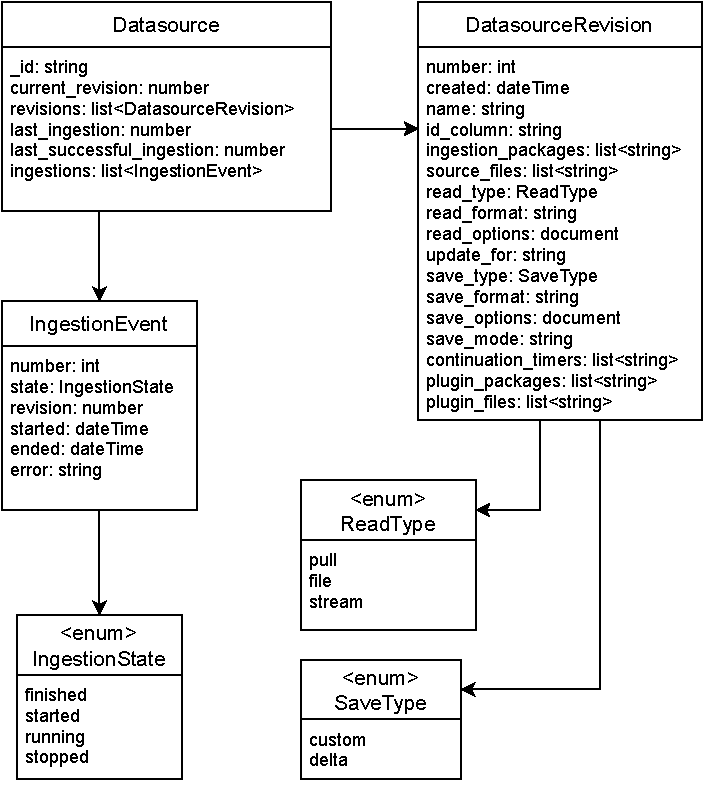
\includegraphics{Grafiken/ingestion-Datamodel.pdf}
    \caption{Datenmodell der Datenquelle}
    \label{fig:datasource_model}
\end{figure}

\subsection{Api-Server}

Da auch das Masterprojekt eine REST-Schnittstelle hat, bietet es sich an, diesen Server so zu erweitern, dass er als Api-Server für das neue System fungiert.
Um die neuen Endpunkte in die aktuelle Lösung zu integrieren, werden die existierenden Pfade, bis auf die zur Authentifizierung, nach "`/api/v1/"' verschoben und die neuen unter "`/api/v2/"' eingefügt.
Auf Grund der Tatsache, dass das neue System mit einem eigenen Datenmodell arbeitet, ist damit die Integration bereits abgehandelt, es muss nur darauf geachtet werden, die Funktionen der beiden Versionen zu trennen.
Die Endpunkte werden mit ihren Funktionen, wie in \fref{sec:arch} beschrieben, implementiert.

Bei der Erstellung und dem Aktualisieren von Datenquellen werden jedes mal eine neue Revision 
Dabei muss besonders darauf geachtet werden, dass bei jeder Änderung einer \verb|Datasource| eine neue \verb|DatasourceRevision| angelegt wird.
Die Quell- oder Plugindateien werden zentral im \textit{HDFS} jeweils einem Unterordner pro Datenquelle abgelegt.
So sind die Dateien von überall aus erreichbar und können auch bei replizierten oder verteilten Microservices verwendet werden.


\subsection{Ingestion-Server}



\subsection{Continuation-Server}

\section{Deltaerkennung}

\section{Datenversionierung}


\newpage
% \bibliographystyle{unsrtnat}
% \bibliography{literatur}

\printbibliography

\end{document}
